% This file was created by tikzplotlib v0.9.4.
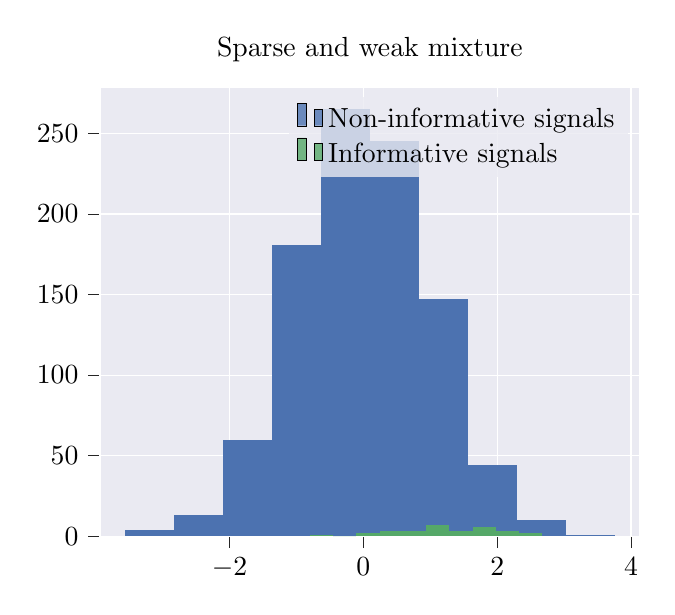
\begin{tikzpicture}

\definecolor{color0}{rgb}{0.917647058823529,0.917647058823529,0.949019607843137}
\definecolor{color1}{rgb}{0.298039215686275,0.447058823529412,0.690196078431373}
\definecolor{color2}{rgb}{0.333333333333333,0.658823529411765,0.407843137254902}

\begin{axis}[
axis background/.style={fill=color0},
axis line style={white},
legend cell align={left},
legend style={fill opacity=0.8, draw opacity=1, text opacity=1, draw=none, fill=color0},
tick align=outside,
tick pos=left,
title={Sparse and weak mixture},
x grid style={white},
xmajorgrids,
xmin=-3.93683926803632, xmax=4.12856704333185,
xtick style={color=white!15!black},
y grid style={white},
ymajorgrids,
ymin=0, ymax=278.25,
ytick style={color=white!15!black}
]
\draw[draw=none,fill=color1,line width=0.12pt] (axis cs:-3.57022989024686,0) rectangle (axis cs:-2.83701113466794,4);
\addlegendimage{ybar,ybar legend,draw=none,fill=color1,line width=0.12pt};
\addlegendentry{Non-informative signals}

\draw[draw=none,fill=color1,line width=0.12pt] (axis cs:-2.83701113466794,0) rectangle (axis cs:-2.10379237908901,13);
\draw[draw=none,fill=color1,line width=0.12pt] (axis cs:-2.10379237908901,0) rectangle (axis cs:-1.37057362351009,60);
\draw[draw=none,fill=color1,line width=0.12pt] (axis cs:-1.37057362351009,0) rectangle (axis cs:-0.637354867931162,181);
\draw[draw=none,fill=color1,line width=0.12pt] (axis cs:-0.637354867931162,0) rectangle (axis cs:0.0958638876477624,265);
\draw[draw=none,fill=color1,line width=0.12pt] (axis cs:0.0958638876477624,0) rectangle (axis cs:0.829082643226687,245);
\draw[draw=none,fill=color1,line width=0.12pt] (axis cs:0.829082643226687,0) rectangle (axis cs:1.56230139880561,147);
\draw[draw=none,fill=color1,line width=0.12pt] (axis cs:1.56230139880561,0) rectangle (axis cs:2.29552015438454,44);
\draw[draw=none,fill=color1,line width=0.12pt] (axis cs:2.29552015438454,0) rectangle (axis cs:3.02873890996346,10);
\draw[draw=none,fill=color1,line width=0.12pt] (axis cs:3.02873890996346,0) rectangle (axis cs:3.76195766554239,1);
\draw[draw=none,fill=color2,line width=0.12pt] (axis cs:-0.800722024704306,0) rectangle (axis cs:-0.453136738259853,1);
\addlegendimage{ybar,ybar legend,draw=none,fill=color2,line width=0.12pt};
\addlegendentry{Informative signals}

\draw[draw=none,fill=color2,line width=0.12pt] (axis cs:-0.453136738259853,0) rectangle (axis cs:-0.105551451815399,0);
\draw[draw=none,fill=color2,line width=0.12pt] (axis cs:-0.105551451815399,0) rectangle (axis cs:0.242033834629055,2);
\draw[draw=none,fill=color2,line width=0.12pt] (axis cs:0.242033834629055,0) rectangle (axis cs:0.589619121073508,3);
\draw[draw=none,fill=color2,line width=0.12pt] (axis cs:0.589619121073508,0) rectangle (axis cs:0.937204407517962,3);
\draw[draw=none,fill=color2,line width=0.12pt] (axis cs:0.937204407517962,0) rectangle (axis cs:1.28478969396242,7);
\draw[draw=none,fill=color2,line width=0.12pt] (axis cs:1.28478969396242,0) rectangle (axis cs:1.63237498040687,3);
\draw[draw=none,fill=color2,line width=0.12pt] (axis cs:1.63237498040687,0) rectangle (axis cs:1.97996026685132,6);
\draw[draw=none,fill=color2,line width=0.12pt] (axis cs:1.97996026685132,0) rectangle (axis cs:2.32754555329578,3);
\draw[draw=none,fill=color2,line width=0.12pt] (axis cs:2.32754555329578,0) rectangle (axis cs:2.67513083974023,2);
\end{axis}

\end{tikzpicture}
